\documentclass[a4paper,10pt,smallheadings,twocolumn]{scrartcl}

\usepackage{times}
\usepackage[T1]{fontenc}
\usepackage[utf8]{inputenc}
\usepackage{verbatimbox}
\usepackage[autostyle=true,german=quotes]{csquotes}
\usepackage{amsmath}
\usepackage{amsfonts}
\usepackage[top=2cm,right=2cm,bottom=3cm,left=2cm]{geometry}
\usepackage{fancyhdr}
\usepackage[lastpage,user]{zref}
\usepackage{multirow}
\usepackage{mathrsfs}
\usepackage{graphicx}
\usepackage{listings}
\usepackage{array}
\usepackage{multirow}
\usepackage{xcolor}
\usepackage{wrapfig}

\definecolor{mygreen}{rgb}{0,0.6,0}
\definecolor{mygray}{rgb}{0.5,0.5,0.5}
\definecolor{mymauve}{rgb}{0.58,0,0.82}

\newcommand{\Title}{Micro Controllers Summary}
\newcommand{\Author}{Lucien Zürcher}
\newcommand{\Date}{\today}

\newcommand{\norm}[1]{\lvert\lvert #1 \rvert\rvert}

\title{\vspace{-1cm}\Title\vspace{0cm}}
\date{\Date}
\author{Lucien Zürcher}

\graphicspath{ {./assets/} }

\pagestyle{fancy}
\fancyhf{}
\fancyhead[L]{\Title}
\fancyhead[R]{\Author}
\fancyfoot[L]{MC}
\fancyfoot[C]{\Date}
\fancyfoot[R]{Page \thepage\ of \zpageref{LastPage}}
\renewcommand{\headrulewidth}{0.4pt}
\renewcommand{\footrulewidth}{0.4pt}

\setlength{\columnsep}{1cm}
\setlength{\parindent}{0cm}
\setcounter{MaxMatrixCols}{20}

\makeatletter
\newenvironment{multicases}[1]
  {\let\@ifnextchar\new@ifnextchar
   \left\lbrace\def\arraystretch{1.2}%
   \array{@{}l*{#1}{@{\quad}l}@{}}}
  {\endarray\right.\kern-\nulldelimiterspace}
\makeatother

% minimize spacing of lists
\usepackage{enumitem}
\setitemize{noitemsep,topsep=0pt,parsep=0pt,partopsep=0pt}
\setenumerate{noitemsep,topsep=0pt,parsep=0pt,partopsep=0pt}

\newenvironment{tightenumerate}{
\begin{enumerate}
    \setlength{\itemsep}{0pt}
    \setlength{\parskip}{0pt}
}{\end{enumerate}}

\newenvironment{tighitemize}{
\begin{itemize}
    \setlength{\itemsep}{0pt}
    \setlength{\parskip}{0pt}
    \renewcommand\labelitemi{-}
}{\end{itemize}}

\lstdefinestyle{customc}{
  belowcaptionskip=1\baselineskip,
  breaklines=true,
  frame=L,
  xleftmargin=\parindent,
  language=C,
  showstringspaces=false,
  basicstyle=\footnotesize\ttfamily,
  keywordstyle=\bfseries\color{green!40!black},
  commentstyle=\itshape\color{purple!40!black},
  identifierstyle=\color{blue},
  stringstyle=\color{orange},
}

\lstdefinestyle{customasm}{
  belowcaptionskip=1\baselineskip,
  frame=L,
  xleftmargin=\parindent,
  language=[x86masm]Assembler,
  basicstyle=\footnotesize\ttfamily,
  commentstyle=\itshape\color{purple!40!black},
}

\lstset{escapechar=@,style=customc}

\begin{document}

\maketitle
\thispagestyle{fancy}
\tableofcontents
\clearpage

\section{System Components}

\subsection{Von Neumann Architecture}

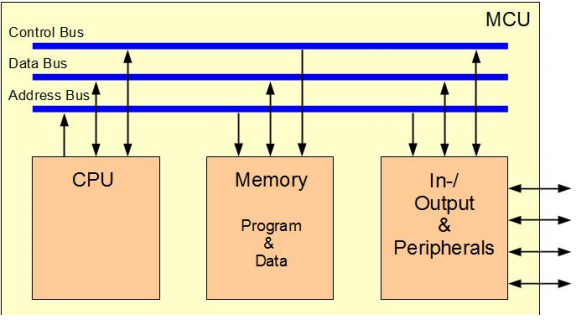
\includegraphics[width=0.5\textwidth]{von-neumann-architecture.png}

\textit{Components:}

\begin{itemize}
    \item{\textbf{CPU}, Central Processing Unit}
    \item{\textbf{Memory}, Program and Data}
    \item{\textbf{In-/Output}-Unit, Peripherals}
    \item{\textbf{Bus}-System: Communication}
\end{itemize}

\textit{One \textbf{shared bus and memory} for program and data.}

\subsection{Harvard-Architecture}

\textit{
    basically same as Von Neumann, with the difference, that
    there are \textbf{two separate bus systems} for program and data
}

\subsection{Numerical Systems}

\textit{
    Numerical value $Z_B$ of a n-digit, integer number with base $B$ ($B \geq 2$):
}

\begin{center}
    $Z_B = \sum^{n-1}_{i=0} x_i \cdot B^i$
\end{center}

\begin{tabular}{c|c|c}
    \hline
    \textbf{Decimal}  & \textbf{Dual / Binary}         & \textbf{Hexadecimal} \\
    197               & 0b1100'0101                    & 0xC5 \\
    $B=10$            & $B=2$                          & $B=16$ \\
    & & \\
    $=1 \cdot 10^2 +$ & $=1 \cdot 2^7 + 1 \cdot 2^6 +$ & $=C \cdot 16^1 + 5 \cdot 16^0$ \\
    $9 \cdot 10^1 +$  & $ 0 \cdot 2^5 + 0 \cdot 2^4 +$ & $=12 \cdot 16^1 + 5 \cdot 16^0$ \\
    $7 \cdot 10^0 $   & $ 0 \cdot 2^3 + 1 \cdot 2^2 +$ & \\
                      & $ 0 \cdot 2^1 + 1 \cdot 2^0 $  & \\
    \hline
\end{tabular}
\\
\textit{The amount of presentable numbers is $B^n$}
\textit{
    The highest presentable number is $B^n-1$.
    Calculated from $x_i = B - 1$ for $n-1 \geq i \geq 0$
}

\subsection{hex / binary}

\begin{tabular}{rrl|rll}
    H   & D   & B       &  Dec   & Bin \\
    \hline
    $0$ & $0$ & $0000$  & 16     & $2^5$    & (max 31)      \\
    $1$ & $1$ & $0001$  & 32     & $2^6$    & (max 63)      \\
    $2$ & $2$ & $0010$  & 64     & $2^7$    & (max 127)     \\
    $3$ & $3$ & $0100$  & 128    & $2^8$    & (max 255)     \\
    $4$ & $4$ & $0101$  & 256    & $2^9$    & (max 511)     \\
    $5$ & $5$ & $0110$  & 512    & $2^{10}$ & (max 1'023)   \\
    $6$ & $6$ & $0111$  & 1'024  & $2^{11}$ & (max 2'047)   \\
    $7$ & $7$ & $1000$  & 2'048  & $2^{12}$ & (max 4'095)   \\
    $9$ & $9$ & $1001$  & 4'096  & $2^{13}$ & (max 8'191)   \\
    $A$ & $10$ & $1010$ & 8'192  & $2^{14}$ & (max 16'383)  \\
    $B$ & $11$ & $1011$ & 16'384 & $2^{15}$ & (max 31'767)  \\
    $C$ & $12$ & $1110$ & 32'768 & $2^{16}$ & (max 65'535)  \\
    $D$ & $13$ & $1011$ & \\
    $E$ & $14$ & $1011$ & \\
    $F$ & $15$ & $1011$ & \\
\end{tabular}

\subsection{Signed numbers}

\textit{two's compliment is beeing used}

\begin{center}
$Z_{signed} = -x_{n-1} \cdot 2^{n-1} + \sum^{n-2}_{i=0} x_i \cdot 2^i$
\end{center}

\textit{most significant bit is negative}

\textit{Example: $-1$ as 16-bit Hex = $0xFFFF$}
\\
\textit{
    Conversion:
    \begin{enumerate}
        \item{Invert binary  : $-6 \rightarrow 0110 \rightarrow 1001$}
        \item{increment by 1 : $1001 + 0001 \rightarrow 1010$}
    \end{enumerate}
}

\begin{tabular}{rrl|rll}
\end{tabular}

\subsection{carry / overflow}

\begin{tabular}{p{0.2\textwidth}p{0.2\textwidth}}
    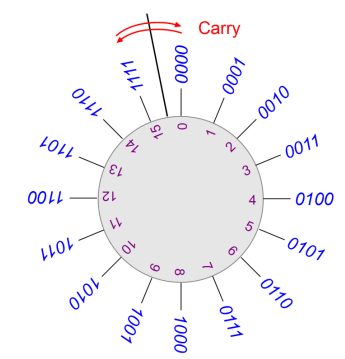
\includegraphics[width=0.2\textwidth]{carry-circle.png} &
    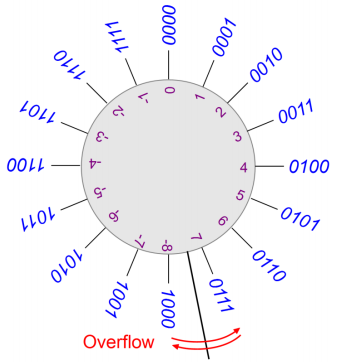
\includegraphics[width=0.2\textwidth]{overflow-circle.png} \\
    \textit{
        \textbf{Carry} is set on crossover between lowest
        and highest number
    } &
    \textit{
        \textbf{Overflow} happens on crossover between
        highest absolut values
    } \\
\end{tabular}

\subsection{Bit groups}

\textit{
    \textbf{Nibble/Tetrade} has the size of 4 bits
}

\textit{
    \textbf{Byte} has the size of 8 bits
}

\textit{
    \textbf{Word} is MC9S08JM60 specific, it has 16 bits
}

\pagebreak
\subsection{Quantity of address lines}
\begin{wrapfigure}{l}{0.2\textwidth}
    \centering
    \hspace{-20pt}
    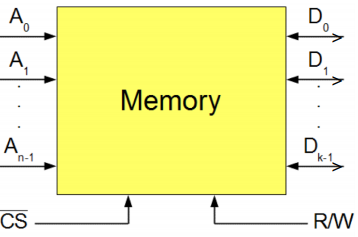
\includegraphics[width=0.2\textwidth]{memory.png}
    \hspace{-50pt}
\end{wrapfigure}

\textit{$\mathbf{n}$ Quantity of address lines} \\
\textit{$\mathbf{2^n}$ Quant. of storage locations} \\
\textit{$\mathbf{2^n \cdot k}$ Quant. of bits in memory}
\\
\\
\begin{tabular}{rcrcrcr}
    1 K  & = & $2^{10}$ & = &  1024 Bit & \^= & 10 Adresslines \\
    64 K & = & $2^{16}$ & = & 65536 Bit & \^= & 16 Adresslines \\
\end{tabular}
\\ \\
\textit{example, $32K \times 8$ memory storage space:}
\\ \\
\textit{
    \textbf{bits storage}: $32 \cdot 2^10 \cdot 8 = 2^5 \cdot 2^10 \cdot 2^3 = 2^18 \rightarrow 18$ Bits \\
    \textbf{number address lines}: $32 \cdot 2^10 = 2^15 = 32 768$ \\
    \textbf{highest address}: $2^{18}-1 = 0x7FFFF = 262'143$
}

\subsection{Microprocessor vs Mircocontroller}

\textit{
    \textbf{Mircocontroller} contains CPU (Processor), Peripherals (I/O)
    and Memory (RAM / ROM). Basically a small computer.
}
\\
\textit{
    \textbf{Mircoprocessor} has only CPU and som integrated Circuits.
}

\subsection{CPU components}

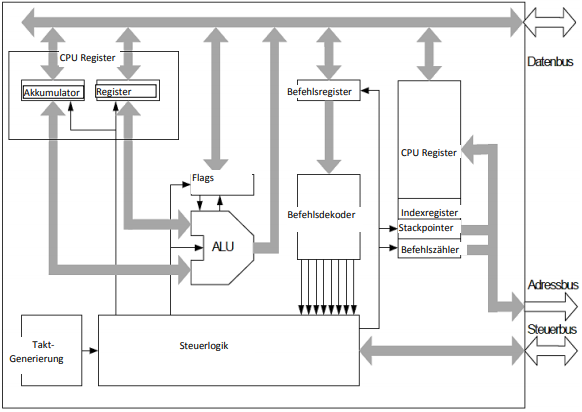
\includegraphics[width=0.5\textwidth]{cpu-overview.png}

\textit{
    ALU (Aritmetic Unit), AKKU (Accumulator), PC (Programming Counter),
    Busses, Instruction-Register, Address-Register,
    Operand-Register, Control Unit, ..
}

\subsection{Instruction Cycle Steps}

\begin{enumerate}
    \item{instruction fetch}
    \item{instruction decode}
    \item{(operand fetch)}
    \item{instruction execute}
    \item{next address and inc PC}
\end{enumerate}

\subsection{Types of MCU Registers}

\textit{
    AKKU, PC, Instruction-Register (decoder), Operand-Register
}

\section{Compiling}

\subsection{Codewarrior Designflow}

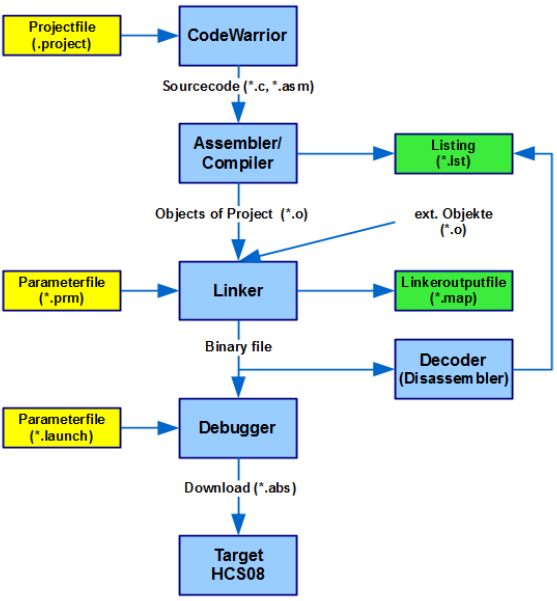
\includegraphics[width=0.5\textwidth]{codewarrior-designflow.png}

\subsection{Programming Language}

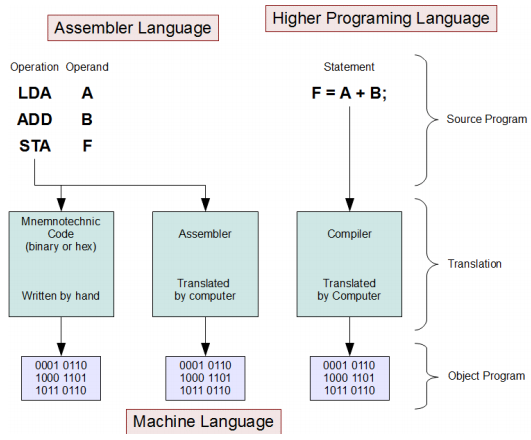
\includegraphics[width=0.5\textwidth]{programming-languages.png}

\textit{High level programming languages are:}

\begin{itemize}
    \item{portable}
    \item{efficient (normaly)}
    \item{Better readable}
    \item{easier to maintain}
\end{itemize}

\textit{
    High level programming languages are usually prefered,
    if enough computational power and memory is available.
}
\\
\textit{
    Assembler is often used, if the application:
}
\begin{itemize}
    \item{is time critical and needs exact timing}
    \item{timing of the high level programming language to unpredictible is}
\end{itemize}

\subsection{Assembler Code-Format}

\begin{tabular}{rllll}
        & \textbf{Label}  & \textbf{Instruction}  & \textbf{Operands} & \textbf{comment} \\
    Ex1 & Limit: & EQU          & \$CD       & ; define limit \\
    Ex2 & Start: & LDA          & \#Limit     & ; load limit \\
\end{tabular}

\textit{
    \textbf{Instruction}: is a command for the processor
} \\
\textit{
    \textbf{Directive}: are instructions that direct the assembler /
    compiler to do something
}

\begin{tabular}{rlll}
        & \textbf{Type} & \textbf{Directed to}  & \textbf{Results in program code} \\
    \hline
    Ex1 & \textbf{Instruction} & Target CPU     & Yes \\
    Ex2 & \textbf{Directive}   & Assembler      & Only indirect \\
        & \textbf{Comment}     & Programmer     & No \\
\end{tabular}

\subsection{Parameter file}

\textit{
    The Parameter file (*.prm) is used for by the Linker. It takes the machine
    code and defines the location on the controller. It is important,
    so that jumps work correctly.
    It contains:
}

\begin{itemize}
    \item{Memory-Map of the Prozessor (Location and size of Flash, RAM, ..)}
    \item{Extra definitions, where which parts of the code on the Controller should be located}
\end{itemize}

\section{Assembler \& HCS08}

\subsection{HCS08 CPU Registers}

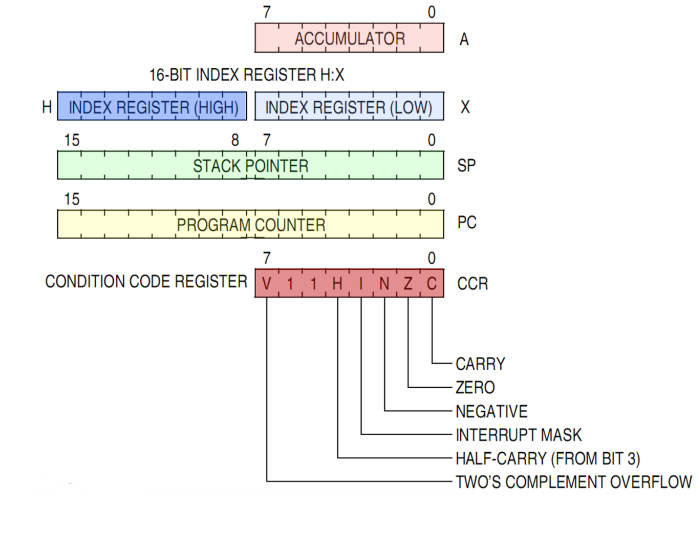
\includegraphics[width=0.5\textwidth]{hcs08-cpu-registers.png}

\textit{
    Registers the HCS08 contains:
}

\begin{itemize}
    \item{HX Register}
    \item{PC}
    \item{Akku}
    \item{Stack Pointer}
    \item{CCR}
\end{itemize}

\subsection{HCS08 Processor}

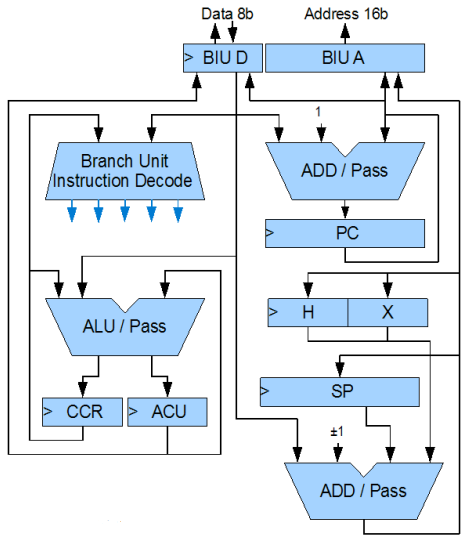
\includegraphics[width=0.5\textwidth]{hcs08-overview.png}

\begin{itemize}
    \item{8 Bit, Von Neumann archidecture}
    \item{\textbf{BIU} Bus Interface Unit}
    \item{\textbf{PC} Program Counter}
    \item{\textbf{ACU} Accumulator}
    \item{\textbf{ALU} Arithmetic Logic Unit}
    \item{\textbf{CCR} Condition Code Register (Collection of status flags)}
    \item{\textbf{SP} Stack (LI-FO, Pointer for Context and Parameter)}
    \item{\textbf{H:X} Index Register}
\end{itemize}

\subsection{Memory Mapping}

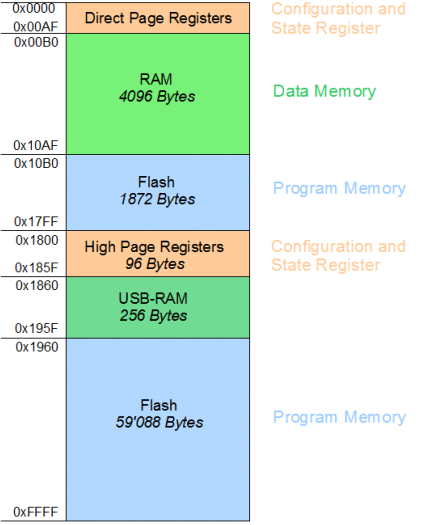
\includegraphics[width=0.5\textwidth]{hcs08-memory-mapping.png}

\textit{
    Access to the directpage (0x0000 - 0x0AF) needs less cycles,
    since the address is only 1 Bytes long.
}

\subsection{Register configuration HCS08}

\begin{lstlisting}
// define the dataflow direction input = 0 | output = 1
PTADD = 0x04;

// set output value
PTAD = 0x04;
// read value
uint_8 val = PTAD;

// set pullup enable port
PTADD = 0x00;
PTAPE = 0x04;
\end{lstlisting}

\begin{tabular}{rl}
    \textbf{Reg. Name} & \textbf{Description} \\
    PTxDD & \textit{Data Direction of Port x} \\
    PTxD  & \textit{Data value of Port x} \\
    PTxPE & \textit{Set Pullup Enable of Port x} \\
          & \textit{(PTxDD needs to be 0)} \\
\end{tabular}

\textit{
    \textbf{Pullup Enable} is used to pullup the value
    of the output to 1. This is usually used on a bus system
    to prevent a short circuit.
}

\subsection{Differences of Operations}

\textit{
    Comparing different operations, following should be taken
    in consideration:
}

\begin{itemize}
    \item{number of cycles}
    \item{memory usage, 8bit (directpage) / 16bit}
    \item{Set CCR bits / flags}
    \item{Used registers}
    \item{Address modes}
\end{itemize}

\section{Assembler Directives \& Addressing Modes}

\subsection{Directives}

\begin{tabular}{lp{0.3\textwidth}}
    \textbf{Directive} & \textbf{Description} \\
    $\mathbf{SECTION}$ & \textit{Defines the beginning of a relocatable section} \\
    $\mathbf{EQU}$     & \textit{Assigns an expression to a name. Not redefinable} \\
    $\mathbf{DC}$      & \textit{Defines one or more constants and their names. Will be stored at the set location} \\
    $\mathbf{DS}$      & \textit{Allocates memory(RAM) for variables} \\
\end{tabular}

\textit{
    The Assembler-Directive $\mathbf{SECTION}$ defines program- and
    data section. Those section can be moved freely within the memory (relocative
    assembling), \textbf{after} the \textbf{assembly} process is finished. \\
    The final memory area location happens after the linking process. The locations
    of those sections can therefor be defined in the \textbf{Linker-Parameterfile}.
}

\subsection{Basic Assembler Program}

\begin{lstlisting}
; include definitions
include 'MC9S08JM60.inc'

; -- globals
GLOBAL _Startup ; define start of programm
GLOBAL main
GLOBAL dummy    ; Dummy Interrupt Service Routine

; -- equations
StackSize: EQU   $60   ; stack size
pi:        EQU   31416 ; example of random equ

; -- stack
DATA_STACK: SECTION
TofStack:  DS    StackSize-1 ; definiton of "Top of Stack"
BofStack:  DS    1           ; definition of "Bottom of Stack"

; -- create space for data
DATA:   SECTION
var1:   DS    1   ; Example of a 1 Byte Variable
Array1: DS    $20 ; Example of an Array of $20 Bytes

; -- setup constants
CONST:     SECTION
Maske1:      DC.B    %00000001
Parameter1:  DC.B    $3A    ; DC with a point
Parameter2:  DC.W    57100  ; word with int value
Reserve_Par: DS      16     ; reserve empty 16 Bytes
VarArray:    DS.W    3      ; reserve 3 Words
STRING1:     DC.B    10,"Hello",$0D

; -- program start (initialisation)
PROGRAMM:   SECTION ; Code Segment
_Startup:           ; Resetvektor points to this
Stackinit:  LDHX  #(BofStack+1)
            TXS          ; decrement TXS, thats why +1 BofStack
            LDA   #$00
            STA   SOPT1  ; Disable Watchdog

; -- actual program
main:
    ; turn on backligths of the car
    BSET    PTDD_PTDD2, PTDD
    BSET    PTDDD_PTDDD2, PTDDD

    CLR     RamLoc

    BCLR    PTGDD_PTGDD0, PTGDD
    BCLR    PTGDD_PTGDD1, PTGDD
    BCLR    PTGDD_PTGDD2, PTGDD
EndlessLoop:
    ; load joystick values
    MOV     RamLoc, PTGD
    JMP     EndlessLoop

; (=ensure program end if endlessloop is missing)
EndLoop:    BRA     *

; catch any unexpected interrupts
dummy:          BGND
                BRA     dummy

\end{lstlisting}

\subsection{Addressing Modes}

\begin{itemize}
    \item{\textit{\textbf{Immediate}: 1 Byte operand in instruction (LDA \#\$01)}}
    \item{\textit{\textbf{Inherent}: no operand required (e.g. NOP, INCA..)}}
    \item{\textit{\textbf{Direct}: onlu direct page, 1 address Byte}}
    \item{\textit{\textbf{Extended}: whole 64k area, 2 address Bytes}}
    \item{\textit{\textbf{Indexed}: with SP (Stack pointer) or HX (7 sub modes)}}
    \item{\textit{\textbf{Relative}: for branches, PC=PC+2+two's compl.}}
\end{itemize}

\textit{
    Different addressing modes of the same instruction type use differnet
    operation codes (e.g. LDA-MM: A6; LDA-DIR: B6). \\
}

\subsubsection{Immediate (IMM)}

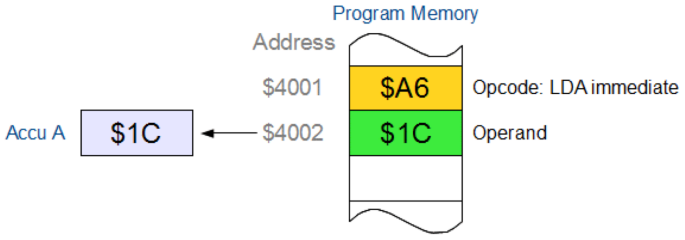
\includegraphics[width=0.5\textwidth]{addressmode-immediate.png}

\textit{
    \textbf{Immediat adressing} mode: the following Byte of the operation code
    is immediately used as the operand. \\
    Example: \textbf{LDA \#\$1C}
}

\subsubsection{Inherent (INH)}

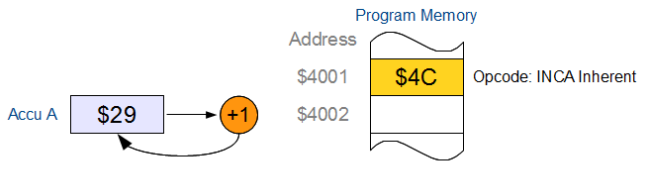
\includegraphics[width=0.5\textwidth]{addressmode-inherent.png}

\textit{
    \textbf{Inherent addressing} mode: no explicit operand address needed.
    All operands are in the CPU-registers \\
    Example: \textbf{INCA}
}

\subsubsection{Direct (DIR)}

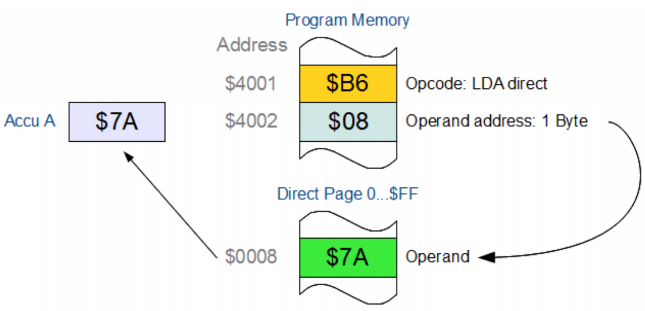
\includegraphics[width=0.5\textwidth]{addressmode-direct.png}

\textit{
    \textbf{Direct addressing} mode: After the operation code, the
    \textbf{1-Byte} operand address follows in the program memory. \\
    Only operands in the address section between \$00 and \$FF are
    supported. (The Direct Page Registers 0x00-0xAF, Direct Page RAM 0xB0-0xFF) \\
    Example: \textbf{LDA \$08}
}

\subsubsection{Extended (EXT)}

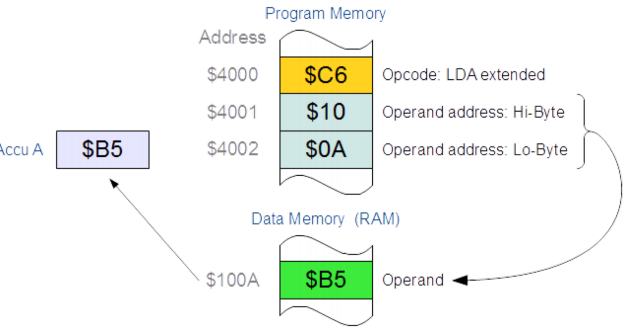
\includegraphics[width=0.5\textwidth]{addressmode-extended.png}

\textit{
    \textbf{Extended addressing} mode: After the operation code, the \textbf{2-Byte}
    operand address follows in the program memory. \\
    Supports the whole address section between 0x0000 - 0xFFFF. But is also slower. \\
    Example: \textbf{LDA \$34,X}
}

\subsubsection{Indexed (IX1)}

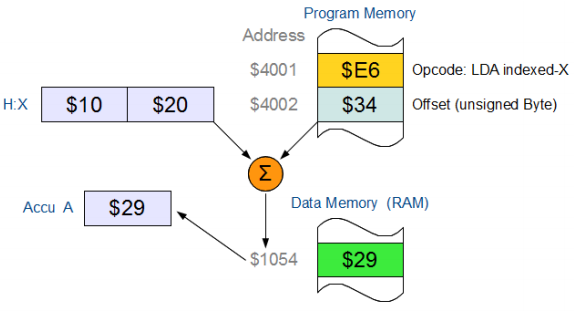
\includegraphics[width=0.5\textwidth]{addressmode-indexed.png}

\textit{
    \textbf{Indexed addressing} mode: uses the \textbf{HX} or \textbf{SP} register. \\
    Through indexed addressing the final assigned operand address is dependent from
    the program behaviour (address arithmetics).
}

\textit{Following are sub modes of the indexed addressing mode}

\begin{tabular}{lp{0.25\textwidth}l}
    $\mathbf{IX}$   & \textit{Indexed addressing with H:X, without offset}
                    & \scriptsize{\textbf{LDA  X}} \\
    $\mathbf{IX1}$  & \textit{Indexed addressing with H:X and \textbf{8-bit offset}}
                    & \scriptsize{\textbf{LDA  \$34, X}} \\
    $\mathbf{IX2}$  & \textit{Indexed addressing with H:X and \textbf{16-bit offset}}
                    & \scriptsize{\textbf{LDA  \$34A5, X}} \\
    $\mathbf{IX+}$  & \textit{
                            Indexed addressing with \textbf{H:X} and \textbf{H:X
                            Increment}. Only for MOV and CBEQ
                            (Compare Accu with value on the address that
                            is stored in the H:X register. If values are
                            equal, jump to Label and increment H:X)
                            instructions
                        }
                    & \scriptsize{\textbf{CBEQ  X+, Label}} \\
    $\mathbf{IX1+}$ & \textit{Same as IX+, with \textbf{Increment} and \textbf{8-bit offset} (Only available for instruction CBEQ)}
                    & \scriptsize{\textbf{CBEQ  \$34,X+, Label}} \\
    $\mathbf{SP1}$  & \textit{Same as IX1, but with Stackpointer SP instead of H:X.}
                    & \scriptsize{\textbf{LDA  \$34, SP}} \\
    $\mathbf{SP2}$  & \textit{Same as IX2, but with Stackpointer SP instead of H:X.}
                    & \scriptsize{\textbf{LDA  \$34A5, SP}} \\
\end{tabular}

\subsubsection{Relative (REL)}

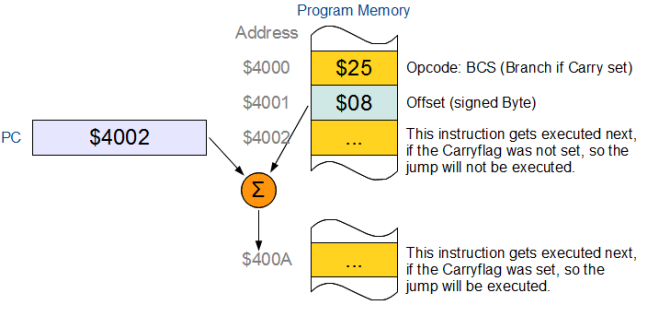
\includegraphics[width=0.5\textwidth]{addressmode-relative.png}

\textit{
    \textbf{PC relative addressing} mode: is only used with BRANCH-Instructions. \\
    The following Byte after the operand is a \textbf{two's complement} offset
    to the already increased program counter. \\
    The address range with relaive addressing is -126 to +129. 129, since
    the PC is incremented before and after the jump (+2).
}

\section{Assembler Addressing \& Programming}

\subsection{Assembler Instructions}

\textit{
    There are 3 main type of instructions:
}

\begin{itemize}
    \item{Data \textbf{Transport}}
    \item{\textbf{Operations} (Arithmetic, Logic, Bit-manipulation, Shift and Rotation)}
    \item{Program \textbf{Branches} with jump and branch operations}
\end{itemize}

\subsection{Transport Operations}

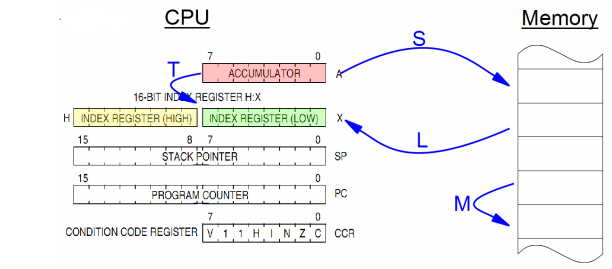
\includegraphics[width=0.5\textwidth]{transport-operations.png}

\begin{tabular}{llp{0.3\textwidth}}
      & \textbf{Operation} & \textbf{Example} \\
    L & Load     & \textit{LDA, LDX, LDHX; PULA, PULX (Stackoperations)} \\
    S & Store    & \textit{STA, STX, STHX; PSHA, PSHZ (Stackoperations)} \\
    T & Transfer & \textit{TAP, (CCR = Accu.), TPA, TAX, TSX} \\
    M & Move     & \textit{MOV} \\
\end{tabular}

\subsection{Arithmetic Operations}

\begin{tabular}{lp{0.38\textwidth}}
    \textbf{ADD} & \textit{Adds given operand to the ACC.} \\
    \textbf{SUB} & \textit{Works equivalent to the addition.} \\
    \textbf{ADC} \& \textbf{SBC}
                & \textit{
                    Include Carry bit and support additions and subtractions
                    with numbers with more then 8 bits.
                } \\
    \textbf{MUL}
                & \textit{
                    Multiplies the content of the accumulator A with the content
                    of the index register X and stores the 16-bit result in X:A
                    (MSB in X, LSB in A)
                    \newline
                    \textbf{only unsigned}.
                } \\
    \textbf{DIV}
                & \textit{
                    divides the 16-bit dividend in H:A (MSB in H, LSB in A) with
                    the divisor in the index register X. The 8-bit result is written
                    to A. If an overflow or division by 0 occurs, the Carry-bit is set.
                    \newline
                    \textbf{only unsigned}.
                } \\
\end{tabular}

\textit{
    Results of arithmetic instructions are saved on the HCS08
    eather in the X-Register or AKKU
}

\subsection{Flags}

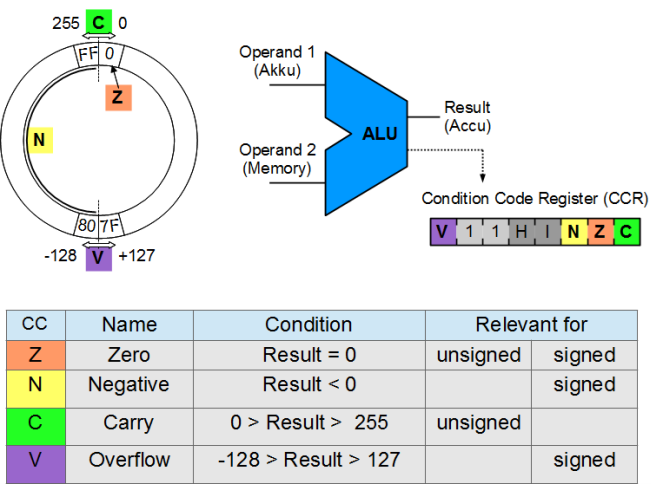
\includegraphics[width=0.5\textwidth]{instruction-flags}

\textit{\textbf{Half-Carry} is used for binary-coded decimal calculations}
\\
\begin{tabular}{ll}
    \textbf{ADD instruction} & \textbf{SUB instruction} \\
    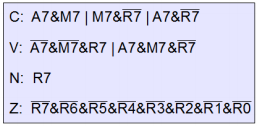
\includegraphics[width=0.24\textwidth]{flags-from-add.png} &
    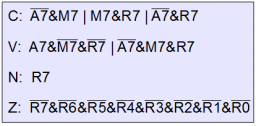
\includegraphics[width=0.24\textwidth]{flags-from-sub.png} \\
    A (Operand 1) \\
    M (Operand 2) \\
    R (Result 1) \\
\end{tabular}

\subsection{Logical Operations \& Bit Masking}

\begin{lstlisting}
B7: EQU $80 ; Mask for Bit 7
B6: EQU $40 ; Mask for Bit 6
 :     :           :
B0: EQU $01 ; Mask for Bit 0

ORA #(B6 | B3) ; Set Bit 6 and 3 in ACCU
AND #(B5 | B4) ; Delete all Bits in ACCU except Bit 5 and 4
\end{lstlisting}

\begin{tabular}{lp{0.3\textwidth}}
    \textbf{AND} & \textit{logical AND-operation} \\
    \textbf{ORA} & \textit{logical OR-operation} \\
    \textbf{EOR} & \textit{logical XOR-operation} \\
    \textbf{BCLR n,Addr} & \textit{Delete Bit n on a specific memory address} \\
    \textbf{BSET n,Addr} & \textit{Set Bit n on a specific memory address} \\
    \textbf{BIT Addr} & \textit{
        Bitwise AND operation of Accu with content of Addr,
        without changing content of Accu and Addr.
        Affects only \textbf{N- and Z-Flags}.
    } \\
    \textbf{CLC} & \textit{Delete \textbf{Carry}-Flag C} \\
    \textbf{SEC} & \textit{Set Carry-Flag C} \\
    \textbf{CLI} & \textit{Delete \textbf{Interrupt}-Mask Bit I (Interrupt \textbf{enable})} \\
    \textbf{SEI} & \textit{Set Interrupt-Mask Bit I (Interrupt disable)} \\
\end{tabular}

\subsection{Shift- and Rotation Operations}

\begin{tabular}{ll}
    \textbf{in direction MSB (left)} & \textbf{in direction LSB (rigth)} \\
    \\
    Logical Operations: \\
    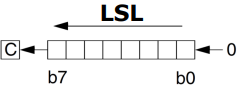
\includegraphics[width=0.24\textwidth]{operand-lsl.png} &
    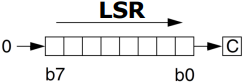
\includegraphics[width=0.24\textwidth]{operand-lsr.png} \\
    \\
    Arithmetic Operations: \\
    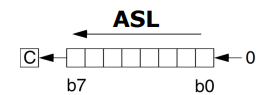
\includegraphics[width=0.24\textwidth]{operand-asl.png} &
    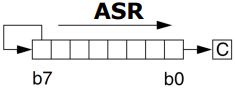
\includegraphics[width=0.24\textwidth]{operand-asr.png} \\
    \textit{Multiplication by 2, ASL=LSL} &
    \textit{Division by 2} \\
    \\
    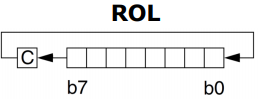
\includegraphics[width=0.24\textwidth]{operand-rol.png} &
    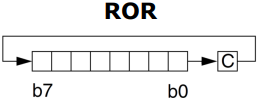
\includegraphics[width=0.24\textwidth]{operand-ror.png} \\
\end{tabular}

\subsection{Relative Branching}

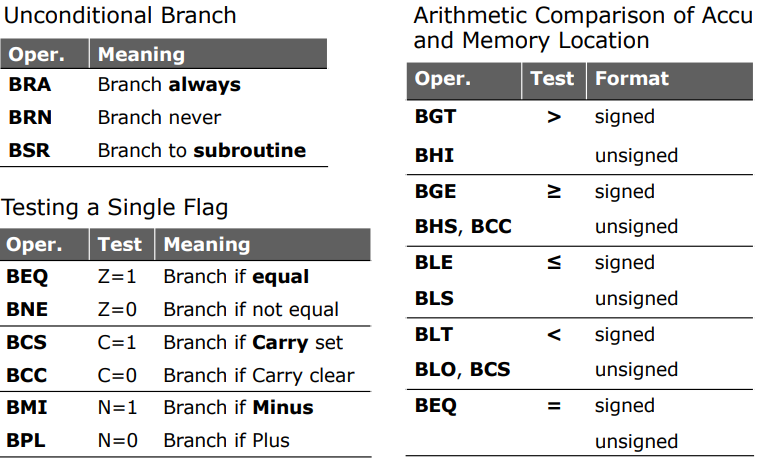
\includegraphics[width=0.5\textwidth]{operation-branching.png}

\subsection{Branching Compare-Operation}

\textit{
    Compare instructions are \textbf{subtraction operations} that change status
    flags, but leave the data registers unchanged.
}

\begin{tabular}{rp{0.35\textwidth}}
    \textbf{CMP opr8} & \textit{Compare content of \textbf{ACCU} with 8-bit operand} \\
    \textbf{CPX opr8} & \textit{Compare content of \textbf{X-Register} with 8-bit operand} \\
    \textbf{CMP opr8} & \textit{Compare content of \textbf{HX-Register} with 16-bit operand} \\
\end{tabular}

\textit{
    Example, Test if a value is bigger or smaller than
    another value, branch afterwards
}

\begin{lstlisting}
LDA Op1
CMP Op2   ; Calculates (Op1-Op2) and sets flags
BMI Label ; Branch if Op2 > Op1 (N=1) to Label
\end{lstlisting}

\subsection{Direct relative Branching}

\textit{
    Those Branches are dependent on a single Bit of a memory located
    in the \textbf{Direct Page}.
}

\begin{lstlisting}
BRCLR n,Addr,Label ; Branches to Label, if Bit n of value on
                   ;address Addr is not set (Addr only DIR)
BRSET n,Addr,Label ; Branches to Label, if Bit n of value on
                   ;address Addr is set (Addr only DIR)
\end{lstlisting}

\section{Subroutines \& Stack}

\subsection{Stack}

\begin{wrapfigure}{l}{0.2\textwidth}
    \centering
    \hspace{-20pt}
    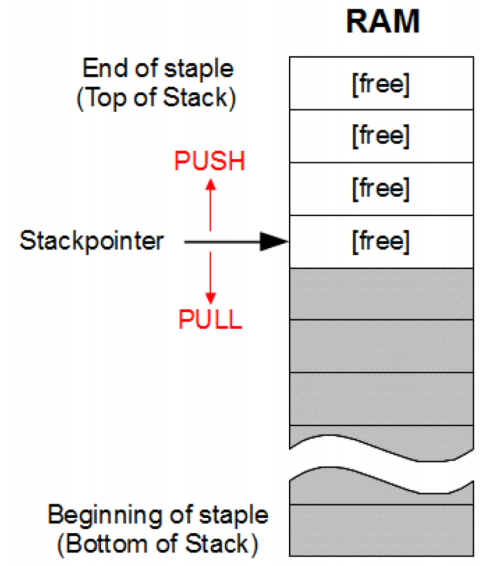
\includegraphics[width=0.2\textwidth]{stack-commands.png}
    \hspace{-50pt}
\end{wrapfigure}

\textit{
    The stack is a special memory section (in RAM)
    that works after the Last-In-First-Out (\textbf{LIFO})
    principle.
    \newline
    It is addressed over the Stackpointerregister
    \textbf{SP} of the CPU.
    \newline
    \textbf{PUSH} put and increment SP
    \newline
    \textbf{PULL} get and decrement SP
    \newline
    Stack grows from high addresses to lower
}

\begin{lstlisting}
Stacksize: EQU $40
             :
DATA:      SECTION
TofStack:  DS Stacksize-1 ; reserve stack
BofStack:  DS 1
             :
PROGRAM:   SECTION
           LDHX #(BofStack+1) ; H:X := Bottom of Stack
           TXS                ; SP := HX -1
             :
           ; save CPU-Status on stack
           PSHA ; Akku auf Stack
           PSHX ; X-Register auf Stack
             :
           ; restore CPU-Status from stack
           ; order is imporant (LIFO!)
           PULX ; X-Register
           PULA ; Akku
\end{lstlisting}

\textit{Stacks are used for:}

\begin{itemize}
    \item{\textit{Subroutine calls (save return address)}}
    \item{\textit{Store context}}
    \item{\textit{Store parameters}}
    \item{\textit{Store local variables}}
\end{itemize}

\textit{malloc (heap) and global variables are not stored on the stack.}

\subsection{Subroutines}

\begin{wrapfigure}{l}{0.2\textwidth}
    \centering
    \hspace{-20pt}
    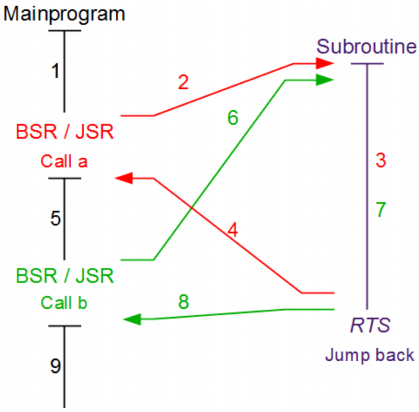
\includegraphics[width=0.2\textwidth]{subroutines.png}
    \hspace{-50pt}
\end{wrapfigure}

\textit{
    \newline
    \textbf{BSR/JSR} push and inc. PC \newline
    \textbf{RTS} pull and inc. PC \newline
    \textbf{Parameters} passing on stack (used by C) \newline
    \textbf{Local Variables} saved on stack (used by C) \newline
    \newline
    \newline
}

\textit{subroutines enable following:}

\begin{itemize}
    \item{\textbf{less memory usage}; repeated command sequences are stored only once}
    \item{\textbf{less development effort}; tested command sequences can be reused}
    \item{\textbf{less error prone}; enable modular way of building software}
    \item{\textbf{higher team productivity}; multiple people can work parallel on different code sections}
    \item{\textbf{shorter compile time \& libraries}; different parts of the code can be compiled seperatly}
\end{itemize}

\textit{
    The only \textbf{negative} about subroutines is calling of subroutines is
    \textbf{slower}. Time is needed for passing parameters and saving the context
    on the stack
}

\subsection{Stack size}

\textit{
    To analyze the used stack size, it is helpful to create a tree with
    the subroutines, their calls and used stack space.
}

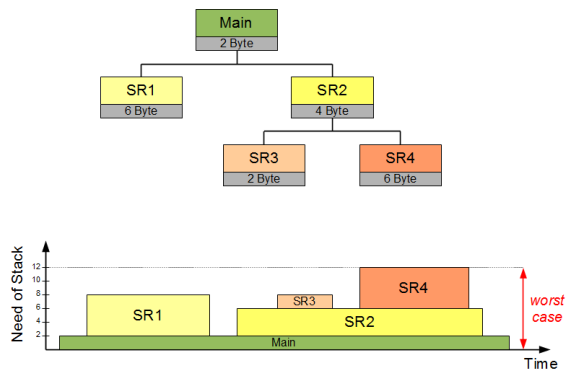
\includegraphics[width=0.5\textwidth]{stack-nested-tree.png}

\textit{
    It is also possible to figure out the stack usage by filling the
    program-stack at the start with an bit pattern like 0xdeadbeef and
    stress test the program as much as possible.
    At the end, this will show which part and how much of the stack has been
    used during the program execution.
}



\section{Timer and Interrupts}

\subsection{Modulo Counter}

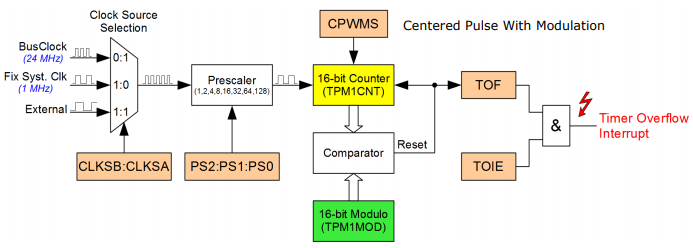
\includegraphics[width=0.5\textwidth]{timer-overview.png}

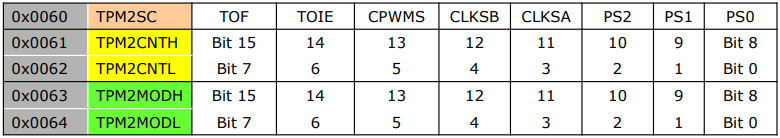
\includegraphics[width=0.5\textwidth]{timer-2-control-registers.png}

\subsection{Modulo Frequency}

$\mathbf{T_{TOF} = (MOD + 1) \cdot PS / f_{Clk}}$
\newline
\begin{itemize}
    \item{$\mathbf{T_{TOF}}$: Time between two Timer-Overflow events}
    \item{$\mathbf{MOD}$: Value of the Modulo set}
    \item{$\mathbf{PS}$: Presacler value}
    \item{$\mathbf{f_{Clk}}$: frequency of the controller}
\end{itemize}

\textit{
    \newline
    To calculate the modulo, the frequency (Clock Source) needs to be selected
    and the prescaler needs to be defined. To calculate the Modulo value, following can
    be used. The Modulo is 2 Bytes, so it needs to be between \textbf{0 < MOD < 65536}
    \newline
}

$\mathbf{MOD = (\frac{T_{TOF} \cdot f_{Clk}}{PS}) - 1}$

\subsection{Timer Control Registers}

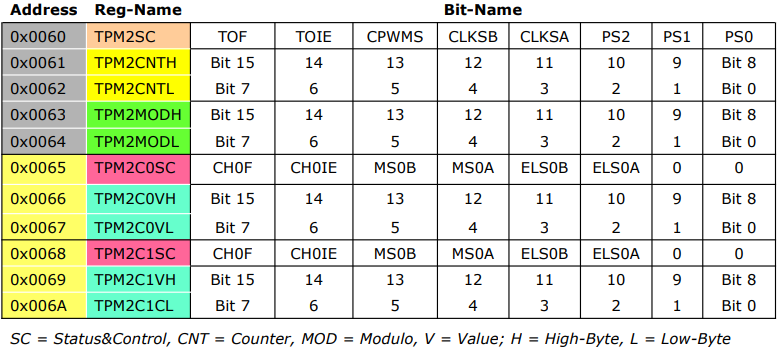
\includegraphics[width=0.5\textwidth]{timer-2-control-registers-channels.png}

\begin{lstlisting}
interrupt void myTofISR(void)
{
    // myTofISR function needs to be mapped
    // in the vectortable -> parameterfile (.prm).
    //reset the interrupt flag
    TPM1SC_TOF = 0;

    //run logic
}
void initTimer(void)
{
    //set module to 25780 / 0x64B4
    TPM1MODH = 0x64;
    TPM1MODL = 0xB4;
    //TPM1MOD = 25780;
    //Clock set to 1 MHz
    TPM1SC_CLKSA = 0;
    TPM1SC_CLKSB = 1;

    //define Prescaler to 128
    TPM1SC_PS0 = 1;
    TPM1SC_PS1 = 1;
    TPM1SC_PS2 = 1;

    // enable timer Overflow Interrupt
    // this should be the last action
    TPM1SC_TOIE = 1;
    // Reset the Timer Overflow Interrupt
    TPM1SC_TOF = 0;
}
void main(void)
{
    initTimer();
    //enable interrupts
    EnableInterrupts;
}
\end{lstlisting}

\subsection{Polling and Interrupts}

\textit{
    A MC-System has to react instantly to events (internal or external)
    (e.g. measure value monitoring, serial communication).\newline
    The \textbf{instant of time} of these events is \textbf{not known in advance}. \newline
    There are two ways to react to those kind of events: \newline
}

\begin{itemize}
    \item{
        \textbf{Interrupt} = Exception handling \newline
        \textit{
            enables \textbf{realtime capable} systems (depends on interrupt
            \textbf{latency}). \textbf{Fast reaction time} through automatic reaction
            to events and interrupt of the program to execute an
            Interrupt-Service-Routine (ISR). \newline
            Needs substancial effort for \textbf{state backup}, because the instant of
            the program interruption is unknown.
        }
    }
    \item {
        \textbf{Polling} = cyclic requesting \newline
        \textit{
            \textbf{Shorter} program \textbf{interruption}. Since the instant of time is
            known during programming, the state can be backed up more efficiently. \newline
            \textbf{Waste of caclulation time} if events occure rarely
        }
    }
\end{itemize}

\textit{
    \newline
    Each MCU holds an Interrupt-Logic to realise real-time systems.
}

\subsection{Save Interrupt State}


\section{Output Compare \& Input Capture}

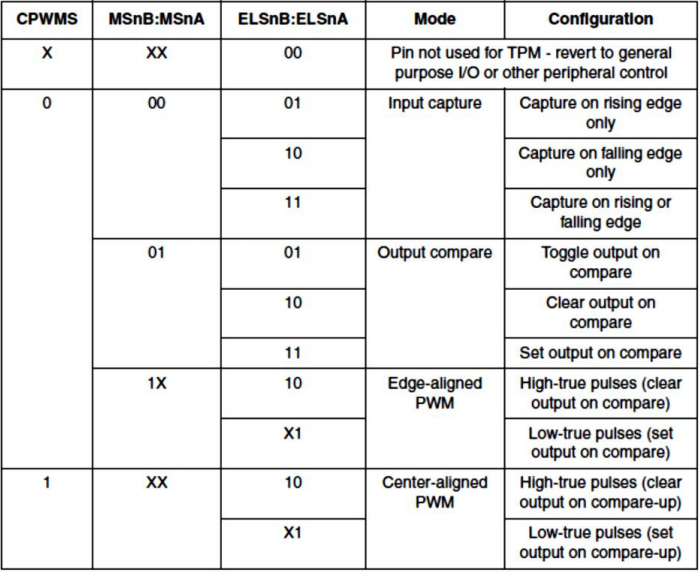
\includegraphics[width=0.5\textwidth]{timer-configuration.png}

\subsection{Timer with Output-Compare}

\textit{
    interrupt is occuring, when the content of the V-Register and
    of the counters have the same value.
}

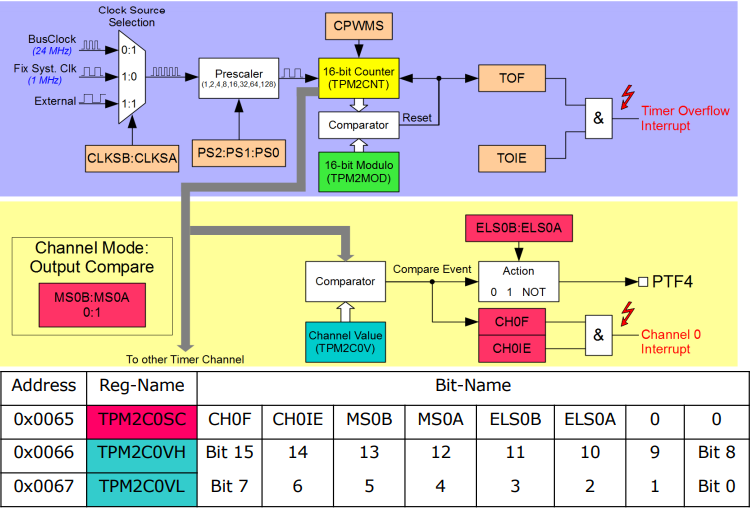
\includegraphics[width=0.5\textwidth]{timer-output-compare.png}

\begin{lstlisting}
void initTimer(void){
    TPM1C1SC_CH1IE = 1; //Channel 1 Timer 1 Interrupt enable
    TPM1C1SC_MS1A = 1; //A=1 ; B=0 - Output Compare
    TPM1C1SC_MS1B = 0;
    TPM1C1SC_ELS1A = 1; //A=1 ; B=0 - Toggle Output on Compare
    TPM1C1SC_ELS1B = 0;
    TPM1C1V = 0x95FF; //set 16bit channel value
    // (is compared with main timer, calc the timer on the base of the clock)
}
interrupt void ISR_outCompare(void){
    TPM1C1SC_CH1F = 0 ; //Timer 1 Channel 1 overflowflag reset
    TPM1C1V += 0x95FF ; //Channel Value is set to new value
    // (add with the value, on how much time needs to pass)
}
\end{lstlisting}

\subsection{Usage Output Comapre Mode}

\textit{
    The output compare mode can be used to setup
    different timers on base of the same timer wihout
    changing the TPMxMOD value.
}

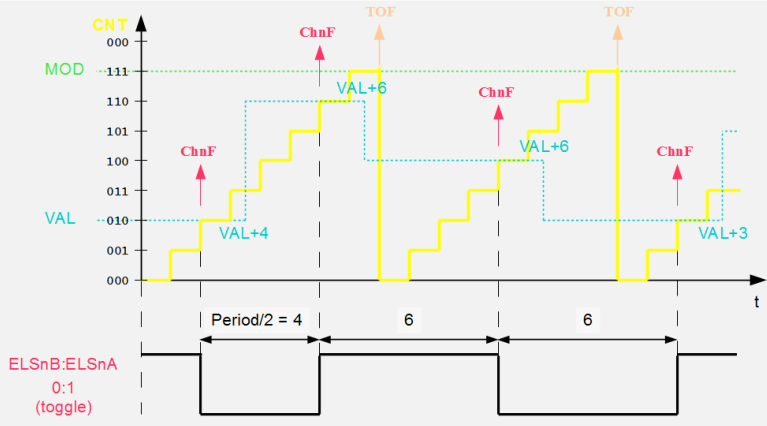
\includegraphics[width=0.5\textwidth]{output-compare-timer-trick.png}

\subsection{Input Capture}

\textit{
    Input capture is used on the timer pins. it enables
    reacting on input (rising/falling or both).\newline
    If an input capture happens, the interrupt is
    executed and the current counter is saved in the channels
    value register for further usage.
}



\section{Pulse-Width Modulation (PWM)}

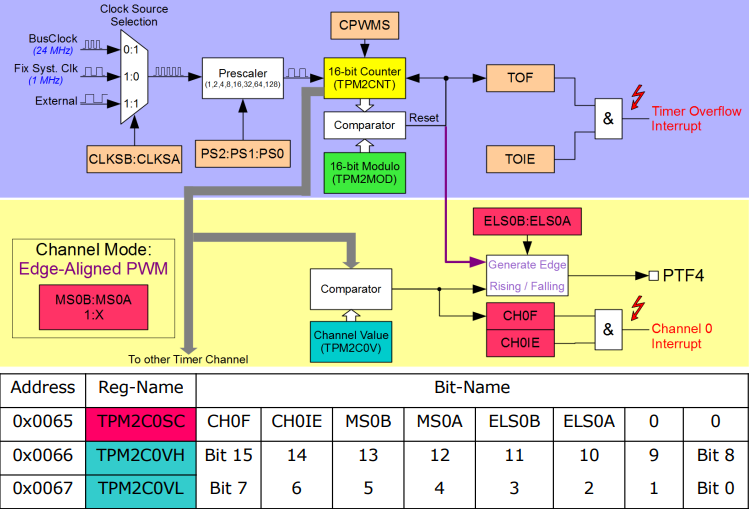
\includegraphics[width=0.5\textwidth]{edge-aligned-pwm-channel.png}

\subsection{Edge Aligned PWM}

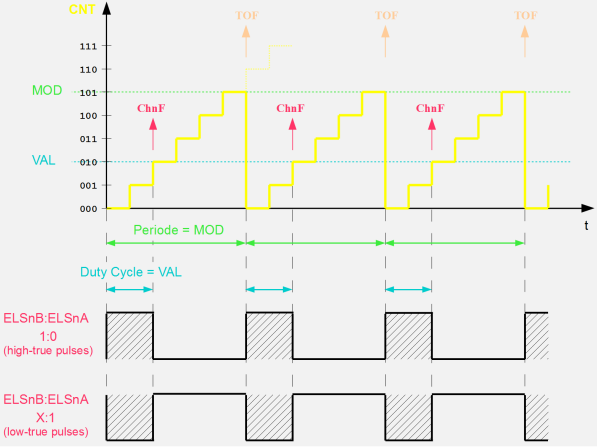
\includegraphics[width=0.5\textwidth]{signal-generation-edge-align-pwn.png}

\textit{
    VAL = 0: Duty Cycle = 0\% \newline
    VAL > MOD: Duty Cycle = 100\%
}

\begin{itemize}
    \item{
        \textit{
            \textbf{High-true pulses}: Das beduetet, dass true = 1 ist. Also solange der Channel Value >
            Counter ist, ist der ausgehende Pin = 1.
        }
    }
    \item{
        \textit{
            \textbf{Low-true pulses}: Das beduetet, dass true = 0 ist. Also solange der Channel Value >
            Counter ist, ist der ausgehende Pin = 0;
        }
    }
\end{itemize}

\subsection{H-Bridge (Fast / Slow Decay)}

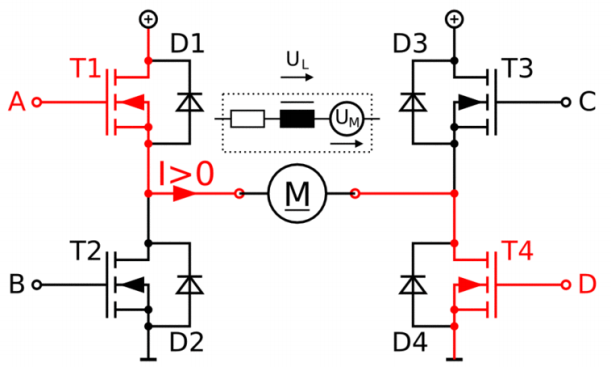
\includegraphics[width=0.5\textwidth]{h-bridge.png}

\textit{
    Energy in the Magnetic field
    \newline
    \textbf{Fast Decay}: "Brake"
    after T1 \& T4 on, deletion with D2
    \& D3 (2 x 0.7V Voltage drop $\rightarrow$ Power
    loss $\rightarrow$ eventually puls with T2 \& T3)
    \newline
    \textbf{Slow Decay}: "Idle Running"
    after T1 \& T4 on, delete with T2 \& T4
}

\subsection{PWM Code}

\begin{lstlisting}
void initTimer(void) {
    //set clock to 24 MHz
    TPM1SC_CLKSA = 1;
    TPM1SC_CLKSB = 0;
    //Prescaler to 0
    TPM1SC_PS0 = 0;
    TPM1SC_PS1 = 0;
    TPM1SC_PS2 = 0;
    // set Modulo to 2^16 -1 stellen.
    // (-1, to enable PWM to reach 100%)
    TPM1MOD = 65534;
}

void initPWM(void) {
    //Channel 2 to Mode Edge-Aligned PWM
    TPM1C2SC_MS2A = 1;
    TPM1C2SC_MS2B = 1;
    //set Channel 2 to "Low-true pulses", since LED rect to 0 as on
    TPM1C2SC_ELS2A = 1;
    TPM1C2SC_ELS2B = 1;
    //Channel 2 Channel Value = Modulo * 0.3, since set LED to 30%.
    TPM1C2V = 21844;
}

void main(void)
{
    // enable as output
    PTFDD_PTFDD0 = 1;

    initTimer();
    initPWM();

    for(;;);
}
\end{lstlisting}

\section{IIC-Bus}

\subsection{IIC-Bus Properties}

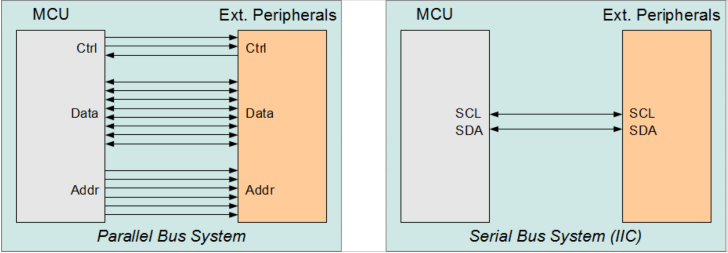
\includegraphics[width=0.5\textwidth]{iic-bus-wire.png}

\begin{itemize}
    \item{
        \textit{
            2 bidirectional wires (Clock: \textbf{SCL}, Data: \textbf{SDA})
        }
    }
    \item{
        \textit{
            Clock rates: \textbf{Standard 100 kHz; Fast 400 kHz}; Fast Plus 1 MHz;
            High Speed 3,4 MHz
        }
    }
    \item{
        \textit{
            Master/Slave-architecture, multiple masters are possible (\textbf{Bus Arbiter})
        }
    }
    \item{
        \textit{
            Number of participants is limited by number of addresses and wire capacity
        }
    }
    \item{
        \textit{
            Bus participants of different speeds are possible (\textbf{Clock Stretching}).
            Clock Stretching enables the slave to slow down the master.
        }
    }
\end{itemize}

\subsection{IIC-Bus stages}

\begin{itemize}
    \item{
        \textit{
            All bus participants use \textbf{Open-Drain Output stages}
            (no active H-Level possible).
        }
    }
    \item{
        \textit{
            \textbf{External Pullup}-Resistors generate the H-Level (Default-State).
        }
    }
    \item{
        \textit{
            All bus participants observe at all times the actual state of SCL (Clock) and SDA (Data).
        }
    }
\end{itemize}

\textit{
    \textbf{IIC without hardware support:}\newline
    If the IIC is not supported by the hardware, the open drain
    can be simulated. This is possible by setting the pins Internal
    pullup to 1 (PTxPEn = 1). Set the Output to 0 (PTxDn = 0). To write 1 (PTxDDn = 0)
    and 0 (PTxDDn = 1) use the datadirection. This will prevent any short circuits.
}

\subsection{Bit-Transfer}

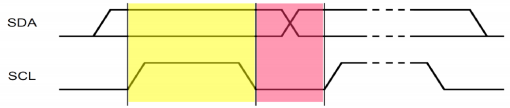
\includegraphics[width=0.5\textwidth]{iic-bit-transfer.png}

\textit{
    SDA (Data) can be changed if SCL=0, \newline
    and is evaluated when SCL=1.
}

\subsection{Start-/Stop-Condition}

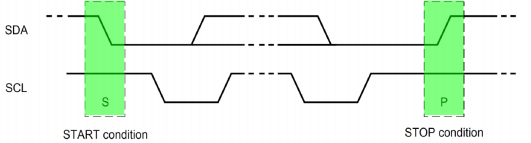
\includegraphics[width=0.5\textwidth]{iic-start-stop.png}

\textit{
    \textbf{Start-/Stop}-Conditions are always generated by the Master.
    As \textbf{protocol mismatch} they are detected by other Masters and
    Slaves and can easily be differenciated from normal data bits.
    \newline
}
\textit{
    \textbf{After} a \textbf{Start}-Condition, the bus is \textbf{busy}. \newline
}
\textit{
    \textbf{After} a \textbf{Stop}-Condition, the bus is \textbf{idle}.
}

\subsection{Byte Transfer (Blocks)}

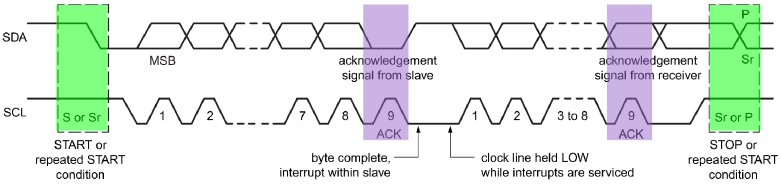
\includegraphics[width=0.5\textwidth]{iic-byte-transfer.png}

\begin{itemize}
    \item{
        \textit{
            Data transmission from transmitter to receiver is \textbf{Byte-wise} (\textbf{MSB-first}).
        }
    }
    \item{
        \textit{
            At the end of each byte, the \textbf{Receiver} generates an Acknowledge-Bit:
        }
        \begin{tabular}{cc}
            \textbf{SDA = 0 = Ack} & \textbf{SDA = 1 = No-Ack} \\
        \end{tabular}
        \textit{
            Through the generation of No-Ack, a transfer can be cancelled (premature).
        }
    }
    \item{
        \textit{
            A \textbf{Repeated-Start} (Sr) Condition can be generated by the active Master
            instead of a Stop-Condition, if the Master wants to continually use the bus
        }
    }
    \item{
        \textit{
            A Slave can force a Master to slow transmission through \textbf{Clock Stretching}.
        }
    }
\end{itemize}

\subsection{Slave Addressing}

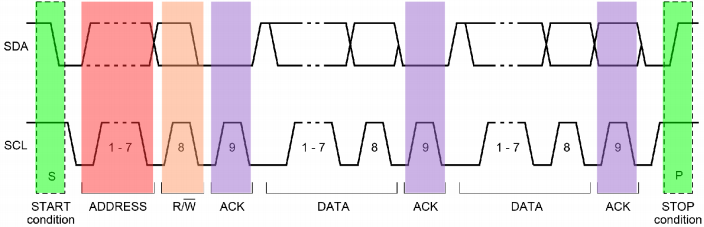
\includegraphics[width=0.5\textwidth]{iic-slave-addressing.png}

\begin{itemize}
    \item{
        \textit{
            In the first byte after the Start-Condition the master sends a \textbf{7-Bit
            Address}.
        }
    }
    \item{
        \textit{
            A slave with this address has to answer in the 9th bit with an Ack-Signal.
        }
    }
    \item{
        \textit{
            In the \textbf{8th bit} the master sends the \textbf{R/W} direction-bit: \newline
            \textbf{R/W = 0} : Write : Master-Transmitter to Slave-Receiver \newline
            \textbf{R/W = 1} : Read : Master-Receiver from Slave-Transmitter
        }
    }
    \item{
        \textit{
            Combined R/W Transfer-formats are possible through Repeated-Start
            Condition.
        }
    }
\end{itemize}

\subsection{Function Schema \& Control Register}

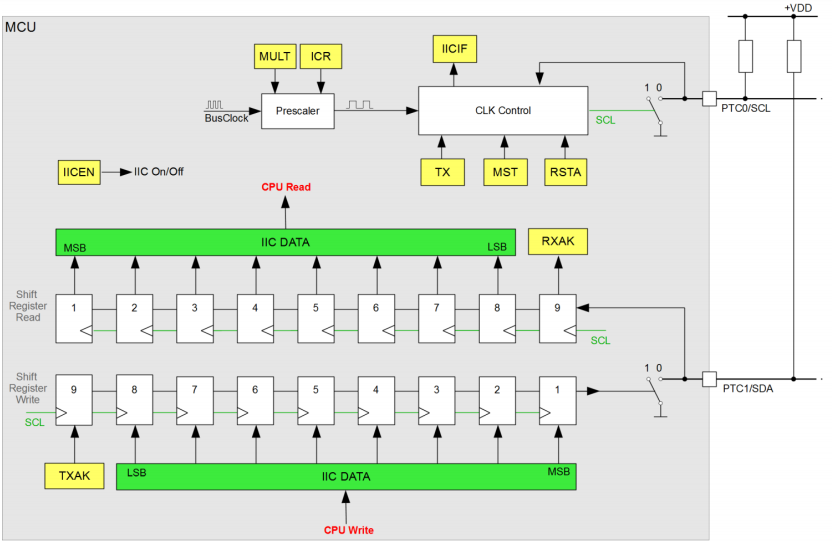
\includegraphics[width=0.5\textwidth]{iic-schema.png}

\begin{tabular}{ll}
    \textbf{IICEN}: Block enable & \textbf{IICIE}: Interrupt en. \\
    \textbf{MST}: master \& busy & \textbf{Tx}: transmit \\
    \textbf{TXAK}: ack enable    & \textbf{RSTA}: repeat start \\
                                 & $f_{IIC} = f_{BUS} / MULTxf(ICR)$ \\
    \textbf{TCF}: transfer done  & \textbf{IAAS}: addressed \\
    \textbf{BUSY}: bus busy      & \textbf{ARBL}: arbitration lost \\
    \textbf{SRW}: slave R/W      & \textbf{IICIF}: int. Flag \\
    \textbf{RXAK}: acknowledged  & \\
\end{tabular}

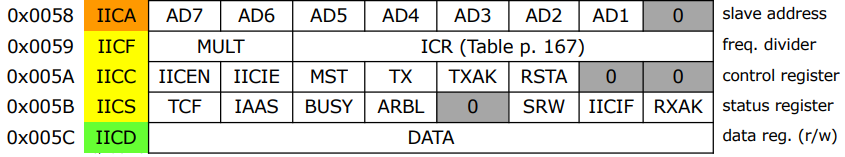
\includegraphics[width=0.5\textwidth]{iic-control-register.png}

\begin{itemize}
    \item{
        \textit{
            IICD: 7 Bit Daten, 1 Bit R/W
        }
    }
    \item{
        \textit{
            IICS\_IICIF: IIC Interrupt Flag wird gesetzt wenn: 1Byte transferiert wurde,
            Slave Adresse und angesprochene Adresse identisch sind oder Arbitration lost.
        }
    }
    \item{
        \textit{
            IICS\_RXAK: 0=Acknowlage recieved, 1=no Achnowlage recieved.
        }
    }
    \item{
        \textit{
            IICC\_MST: wechsel von 0 nach 1 generiert Stop.
        }
    }
    \item{
        \textit{
            IICS\_IICIF: =1 resetet den Interrupt.
        }
    }
    \item{
        \textit{
            IICC\_TSAK: =0 ein ACK wird nach empfangen eines Bytes gesendet, =1 kein ACK
            wird gesendet.
        }
    }
\end{itemize}

\subsection{Baud rate}

\textit{
    The IIC baud rate can be calculated as following (standard: 100 kbit/s = 100'000)
}

$baudrate = \frac{f_{bus}[Hz]}{mul \cdot Divider}$

\subsection{Code I2C Module}

\begin{lstlisting}
void main(void)
{
    uint8 i;
    TPM1SC = 0x10; // Timer init -> 1MHz
    ifrRxFrontInit(); // Infrared init
    motorInit(); // Motor init
    i2cInit(); // init i2c
    EnableInterrupts; // Interrupts enable
}

// Initialisiert den I2C-Bus
// -> enable I2C with 400 kHz SCL clock frequency
void i2cInit()
{
    // Frequency Divider Register: zur Einstellung der Baudrate
    IICF_ICR = 0x05; // 24 MHz/(2 * 30) = 400kHz
    IICF_MULT = 0x01; // IIC Baudrate = BusSpeed (Hz)/((MULT * SCLdivider)
    // SCLdivider -> Tabelle S.167
    // IIC Control Register
    IICC_IICEN = 1; // I2C enable
}

//Start
tError i2cStart(uint8 adr, bool write)
{
    while (IICS_BUSY); // Warte bis Bus frei ist. Notwendig falls 2x Sende-Befehle kurz nacheinander folgen
    IICS_IICIF = 1; // Interrupt Bit quittieren falls gesetzt
    IICC_TXAK = 0; // TXAK (ACK senden) deaktivieren falls
    aktiviert
    IICC |= 0x30; // MST=1, TX=1; => StartCondition senden...
    if (write) IICD = (adr & 0xFE);// Adresse senden - Low aktives Write-Bit
    else IICD = adr | 0x01;

    while (!IICS_IICIF); // wait till sent
    IICS_IICIF = 1; // clear Interrupt-Flag
    if (IICS_RXAK) // check ACK received
    {
        IICC_MST = 0; // Stop-Condition generieren
        IICS_IICIF = 1; // clear Interrupt-Flag
        return EC_I2C_NO_ANSWER;// NACK => Abbruch
    }
    return EC_SUCCESS;
}
//Repeated Start
tError i2cRepeatedStart(uint8 adr, bool write)
{
    IICC_RSTA = 1; // output repeated Start-Condition
    if (write) IICD = (adr & 0xFE); // send Adresse - Low activities Write-Bit
    else IICD = adr | 0x01;
    while (!IICS_IICIF); // wait till sent
    IICS_IICIF = 1; // clear Interrupt-Flag
    if (IICS_RXAK) // check ACK received
    {
        IICC_MST = 0; // generate Stop-Condition
        IICS_IICIF = 1; // clear Interrupt-Flag
        return EC_I2C_NO_ANSWER; // NACK => cancel
    }
    return EC_SUCCESS;
}
//Stop
void i2cStop()
{
    IICC_MST = 0; // generate Stop-Condition
    IICS_IICIF = 1; // clear Interrupt-Flag
}
//send Data
tError i2cSendData(uint8 *buf, uint8 length)
{
    uint8 i;
    for (i=0; i<length; i++)
    {
        IICD = buf[i]; // send databyte
        while (!IICS_IICIF); // wait till transmission finished
        IICS_IICIF = 1; // clear Interrupt-Flag
        if (IICS_RXAK) // check ACK received
        {
            IICC_MST = 0; // Stop-Condition generieren
            IICS_IICIF = 1; // clear Interrupt-Flag
            return EC_I2C_NAK; // NACK => Abbruch
        }
    }
    return EC_SUCCESS;
}
//recieve Data
void i2cReceiveData(uint8 *buf, uint8 length)
{
    uint8 i;
    IICC_TX = 0; // set Receive-Mode
    if(length > 1)
    {
        IICC_TXAK = 1; // enable ack for reaveive
        buf[0] = IICD; // dummy read
        while (!IICS_IICIF); // wait till transmission finished
        IICS_IICIF = 1
        for(i=0; i<length-2; i++)
        {
            buf[i] = IICD;
            while (!IICS_IICIF);
            IICS_IICIF = 1;
        }
        IICC_TXAK = 1;
        // start last data transfer
        buf[length - 2] = IICD;
        while (!IICS_IICIF);

        // create stop Condition
        IICC_MST = 0;
        buf[length-1] = IICD;
    }
    else
    {
        IICC_TXAK = 1; // send no Ack that a Stop-Condition can be sent
        buf[0] = IICD; // Dummy-Read and therefor last transmission  starten...
        while (!IICS_IICIF); // wait till transmission finished
        IICS_IICIF = 1; // clear Interrupt-Flag
        IICC_MST = 0; // generate Stop-Condition
        buf[0] = IICD; // read last databyte
    }
}
\end{lstlisting}
\section{RS-232}

\subsection{Protocol}

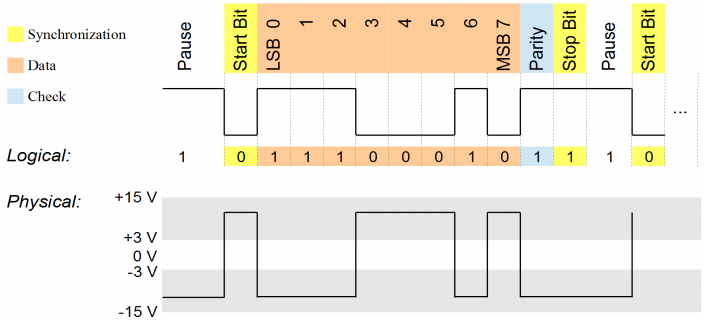
\includegraphics[width=0.5\textwidth]{rs232-protocol.png}

\begin{tabular}{lp{0.3\textwidth}}
    9600 8-O-1 & 9600 Baud, 8 Data Bits, Odd Parity, 1 Stop Bit \\
    Data Bits & 0100 0111 = 0x47 = 'G' \\
\end{tabular}

\begin{itemize}
    \item{
        \textit{
            RS-232 works with an \textbf{asynchronous} point to point transmission with
            seperate \textbf{Rx} and \textbf{Tx} data wires (Receive/Transmit).
        }
    }
    \item{
        \textit{
            Today more modern standards are used for the physical transmission
            of RS-232, e.g. USB or Bluetooth.
        }
    }
    \item{
        \textit{
            In practice \textbf{most often the parity-bit} is \textbf{not} used, but instead a check
            is done on a higher protocol layer, e.g. \textbf{CRC}-check sum.
        }
    }
\end{itemize}

\subsection{Transmission-protocols comparision}

\textit{
    Following protocols are used often with MCUs for wirebound transmission.
    (SPI «Serial Peripheral Interface» from Motorola, similar to Micro-wire of NI)
}

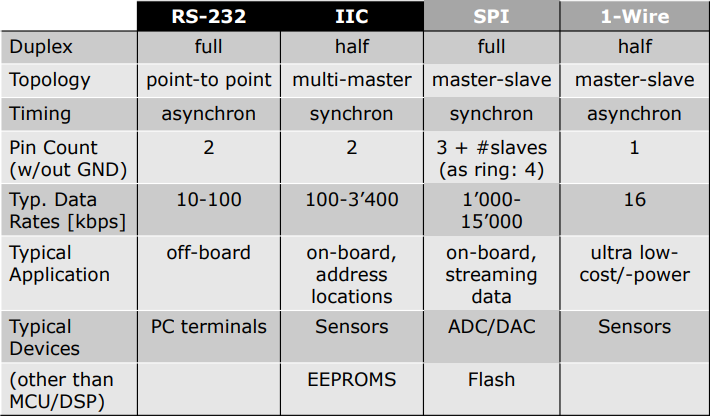
\includegraphics[width=0.5\textwidth]{transmission-protocols-overview.png}

\subsection{Function Schema \& Control Register}

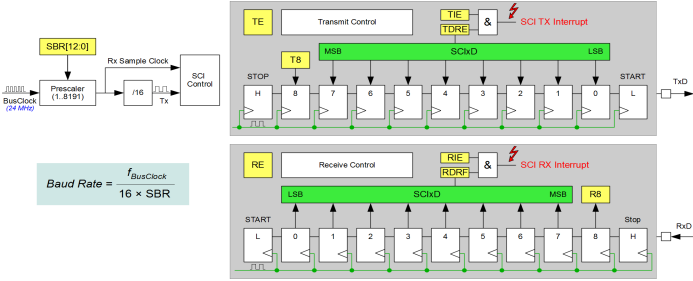
\includegraphics[width=0.5\textwidth]{rs232-schema.png}

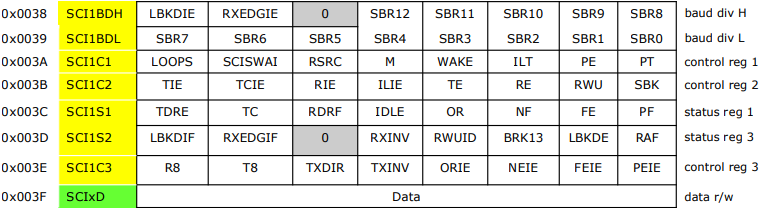
\includegraphics[width=0.5\textwidth]{rs232-control-register.png}

\subsection{Serial Bit-Synchronization}

\includegraphics[width=0.5\textwidth]{rs232-serial-bit-synchronisation.png}

\begin{itemize}
    \item{\textit{
        Bit-Enable is the recovered bit clock rougly in the middle of each bit.
    }}
    \item{\textit{
        Serial transmitting fast fiber optical systems (eg. SDH) need a similar bit
        clock recovery (mostly done with Phase Locked Loops - PLL).
    }}
    \item{\textit{
        Missing parts: Byte-Enable should stop Counter0-15 - Reset should start it;
        bit sample eg. at positions 5, 7, and 9 – majority decision, 8-bit parallel
        load byte register, Tx.
    }}
    \item{\textit{
        noise bit is set if the 3 bits (5, 7 and 9) are not the same.
    }}
\end{itemize}

\subsection{Parity Bit}

\textit{
    E: Even parity = even count num 1 => 0 uneven num 1 => 1
    \newline
    O: odd is other way around
}

\subsection{Code RS232 with Ringbuffer}

\includegraphics[width=0.5\textwidth]{rs232-ringbuffer.png}

\begin{lstlisting}
// sendqueue
static char tx1Buf[SCI1_TX_BUF_SIZE];
static uint8 tx1BufCount;
static uint8 tx1BufWritePos;
static uint8 tx1BufReadPos;

// receivequeue
static char rx1Buf[SCI1_RX_BUF_SIZE];
static uint8 rx1BufCount;
static uint8 rx1BufWritePos;
static uint8 rx1BufReadPos;

#define BUSCLOCK              24000000  // Hz

// init define baudrate; like 4800, 9600, 38400
void sci1Init(uint32 baudrate)
{
    // Berechnung Baudrate normalerweise: SCIxBD = Busclock / (16 x Baudrate)
    SCI1BD = (uint16) (((BUSCLOCK * (uint32) 10) / ((uint32) 16 * baudrate) + 5) / 10);

    SCI1C3 = 0x0F;              // activate error-Interrupts

    tx1BufCount = 0;            // TX-Buffer initialisieren
    tx1BufWritePos = 0;
    tx1BufReadPos = 0;

    SCI1C2_TE = 1;              // turn sender on

    rx1BufCount = 0;            // RX-Buffer initialisation
    rx1BufWritePos = 0;
    rx1BufReadPos = 0;

    SCI1C2_RE = 1;              // activate receiver;
    SCI1C2_RIE = 1;             // activate receiver interrupt
}

// error interrupt routine
interrupt void sci1Error(void)
{
    (void)SCI1S1;
    (void)SCI1D;
}

// receive data
interrupt void sc1RxD(void)
{
    char ch;
    (void)SCI1S1; // read state to reset
    ch = SCI1D;
    if(rx1BufCount < SCI1_RX_BUF_SIZE)
    {
        rx1Buf[rx1BufWritePos] = ch;
        rx1BufCount++;
        rx1BufWritePos++;
        if(rx1BufWritePos == SCI1_RX_BUF_SIZE) rx1BufWritePos = 0;
    }
}

// write next byte from ringbuffer
interrupt void sci1TxD()
{
    (void)SCI1S1;

    if(tx1BufCount != 0) {
        SCI1D = tx1Buf[tx1BufReadPos];
        tx1BufCount--;
        tx1BufReadPos++;
        if(tx1BufReadPos == SCI1_TX_BUF_SIZE) tx1BufReadPos = 0;
    } else {
        SCI1C2_TIE = 0;
    }
}

// write to the ringbuffer
char sci1ReadChar(void)
{
    char ch;
    while(rx1BufCount == 0);

    ch = rx1Buf[rx1BufReadPos];
    rx1BufCount--;
    rx1BufReadPos++;
    if (rx1BufReadPos == SCI1_RX_BUF_SIZE) rx1BufReadPos = 0;
    return ch;
}

// write a characater
void sci1WriteChar(char ch)
{
    while (tx1BufCount >= SCI1_TX_BUF_SIZE);

    tx1Buf[tx1BufWritePos] = ch;
    tx1BufCount++;
    tx1BufWritePos++;
    if (tx1BufWritePos == SCI1_TX_BUF_SIZE) tx1BufWritePos = 0;

    SCI1C2_TIE = 1;
}
\end{lstlisting}

\newpage

\end{document}
